\documentclass[12pt]{article}
\usepackage{graphicx}
\usepackage{amsmath}
\usepackage[framed]{matlab-prettifier}
 \usepackage{pdfpages}
\begin{document}
\begin{titlepage}
	\begin{center}
	\line(1,0){300}\\
	[0.25in]
	\huge{\bfseries Lab 1: Kinematic Characterization of the Lynx (MATLAB)}\\
	[0.12in]
	\line(1,0){200}\\
	[1cm]
	\textsc{\Large University of Pennsylvania}\\
	\end{center}
	\vfill
	\begin{flushright}
	\textsc{\large Wesley Yee, Shaun Fedrick\\
	MEAM 520\\
	September 23, 2020\\}
	\end{flushright}
\end{titlepage}

\section{Methods}
For our experimental setup, we used MATLAB to code our forward kinematics calculations, which communicated to ROS via Gazebo on a local VM running Ubuntu. A 6-DOF robot arm manipulator was programmed to run in Gazebo. Once the code was run in MATLAB on the host computer, the commands for operating the robot were then sent to Gazebo which then actuated the robot to the desired joint variable positions. \\ \\
The ROS robot was modeled off of an actual physical robot located at Penn, but was not accessible due to COVID-19.
\begin{enumerate}
\item \begin{figure} [h]
	\centering 
	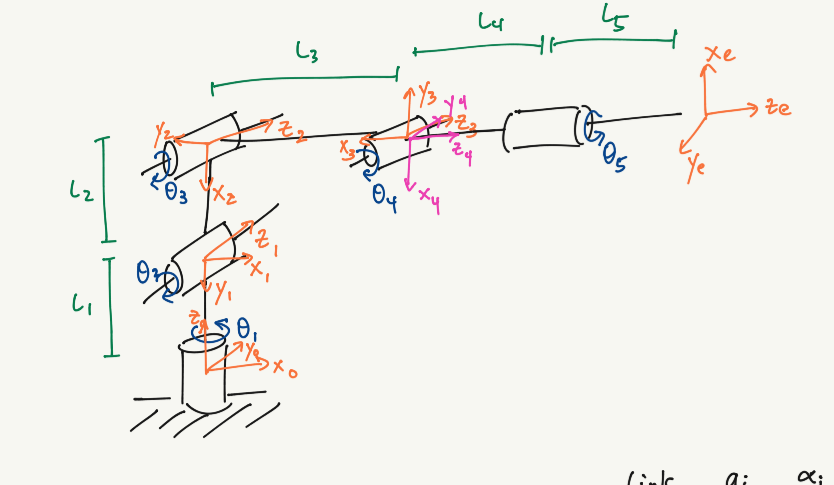
\includegraphics[scale=1]{Q1.png}
	\caption{Revised symbolic representation}
	\end{figure}
\par{ As can be seen from our schematic we chose to use DH4 convention to describe the forward kinematics of our robot.
To do this, we needed to follow the DH4 parameters for each link. This can be seen in the matrix below.}
\begin{equation}
	DH_{4} = \begin{bmatrix}
	Link & a_{i} & \alpha_{i} &d_{i} &\theta_{i}\\
	1&0 & -\frac{\pi}{2} & L_{1}&  \theta_{1}\\
	2&-L_{2}  & 0 & 0 &  \theta_{2}+\frac{\pi}{2}\\
	3&-L_{3} & 0 & 0 & \theta_{3}+\frac{\pi}{2}\\
	4&0 & \frac{\pi}{2} & 0 & \theta_{4}-\frac{\pi}{2}\\
	5(e)&0&0& L_{4}+L_{5}&\theta_{5}+\pi
	\end{bmatrix}
\end{equation}
\par{ It is worth noting that DH parameters work by specifying a Homogeneous transform consisting of a rotation about $\theta_{i}$ along with a translation along $z_{i-1}$. Then from this intermediate frame you perform translation in x by $a_{i}$ along with a final rotation about x by $\alpha_{i}$. Multiplying these transformations gives the homogeneous transform $A^{i-1}_{i}$, we use c to represent cosine and s to represent sine A is given as:}
\begin{equation}
	A^{i-1}_{i} = \begin{bmatrix}
	c_{\theta_{i}} & -s_{\theta_{i}}c_{\alpha_{i}}& s_{\theta_{i}}s_{\alpha_{i}}& a_{i} c_{\theta_{i}}\\
	s_{\theta_{i}} & c_{\theta_{i}}c_{\alpha_{i}}& -c_{\theta_{i}}s_{\alpha_{i}}& a_{i} s_{\theta_{i}}\\
	0 & s_{\alpha_{i}} & c_{\theta_{i}} & d_{i}\\
	0 & 0 & 0 & 1
	\end{bmatrix}
\end{equation}
\item 
\par{ Using $A^{i-1}_{i}$ we get the transformation from consecutive links to be:}
\begin{equation}	
	T^{0}_{1} = \begin{bmatrix}
	c_{\theta_{1}} & 0 & -s_{\theta_{1}}& 0\\
	s_{\theta_{1}}  & 0 & c_{\theta_{1}}& 0\\
	0 & -1 & c_{\theta_{1}}  & L_{1}\\
	0 & 0 & 0 & 1
	\end{bmatrix}
\end{equation}
\begin{equation}	
	T^{1}_{2} = \begin{bmatrix}
	-s_{\theta_{2}} & -c_{\theta_{2}}  & 0 & L_{2}s_{\theta_{2}} \\
	c_{\theta_{2}}  & -s_{\theta_{2}}  & 0& -L_{2}c_{\theta_{2}}\\
	0 & 0 & -s_{\theta_{1}}  & 0\\
	0 & 0 & 0 & 1
	\end{bmatrix}
\end{equation}

\begin{equation}	
	T^{2}_{3} = \begin{bmatrix}
	-s_{\theta_{3}} & -c_{\theta_{3}}  & 0 & L_{3}s_{\theta_{3}} \\
	c_{\theta_{3}}  & -s_{\theta_{3}}  & 0& -L_{3}c_{\theta_{3}}\\
	0 & 0 & -s_{\theta_{3}}  & 0\\
	0 & 0 & 0 & 1
	\end{bmatrix}
\end{equation}

\begin{equation}	
	T^{3}_{4} = \begin{bmatrix}
	s_{\theta_{4}} & 0  & -c_{\theta_{4}}  &0\\
	-c_{\theta_{4}}  & 0  & -s_{\theta_{4}} & 0\\
	0 & 1 & s_{\theta_{4}}  & 0\\
	0 & 0 & 0 & 1
	\end{bmatrix}
\end{equation}

\begin{equation}	
	T^{4}_{5(e)} = \begin{bmatrix}
	-c_{\theta_{5}} & s_{\theta_{5}}   & 0  &0\\
	-s_{\theta_{5}} & -c_{\theta_{5}}  & 0 & 0\\
	0 & 0 & -c_{\theta_{5}} & L_{4}+L_{5}\\
	0 & 0 & 0 & 1
	\end{bmatrix}
\end{equation}

\item 

To get the position of the end effector in terms of the end effector frames all we need to do is post multiply all the matrices from the previous part. Writing out the entirety of this matrix is not feasible, but we can write it in terms of the matrices we are multiplying. This gives:
$T^{0}_{5(e)} =T^{0}_{1}*T^{1}_{2}*T^{2}_{3}*T^{3}_{4}*T^{4}_{5(e)}$
\end{enumerate}
 


\newpage
\section{Evaluation}
\begin{enumerate}
\item The following is the zero joint orientation and location of the end effector. This matrix matches the expected transformation matrix from the pre-lab.
\begin{equation}	
	T^{0}_{e} = \begin{bmatrix}
	0 & 0 & 1 & 255.325mm\\
	0 & -1 & 0 & 0mm\\
	1 & 0 & 0 & 222.25mm\\
	0 & 0 & 0 & 1
	\end{bmatrix}
\end{equation}
\item
\begin{enumerate}
\item The following is the matrix for q = [$pi/4$ 0 0 0 0 0]:
\begin{equation}	
	T^{0}_{e} = \begin{bmatrix}
	0 & \frac{\sqrt{2}}{2} & \frac{\sqrt{2}}{2} & 180.542mm\\
	0 & -\frac{\sqrt{2}}{2} & \frac{\sqrt{2}}{2} & 180.542mm\\
	1 & 0 & 0 & 222.25mm\\
	0 & 0 & 0 & 1
	\end{bmatrix}
\end{equation}
\item The following is the matrix for q = [$-pi/2$ 0 $pi/4$ 0 0 $pi/2$]:
\begin{equation}	
	T^{0}_{e} = \begin{bmatrix}
	-1 & 0 & 0 & 0mm\\
	0 & \frac{\sqrt{2}}{2} & -\frac{\sqrt{2}}{2} & -180.542mm\\
	0 & -\frac{\sqrt{2}}{2} & -\frac{\sqrt{2}}{2} & 41.708mm\\
	0 & 0 & 0 & 1
	\end{bmatrix}
\end{equation}
\end{enumerate}
\item 
\par{
The first interesting configuration we found was done by attempting to make the end effector collide with the base of the robot. This was very possible despite it being within the joint limits, and this was done by imputing  q=[0,0,1.5882,1.700,0,0].  
}  \\
\begin{figure} [h]
	\centering 
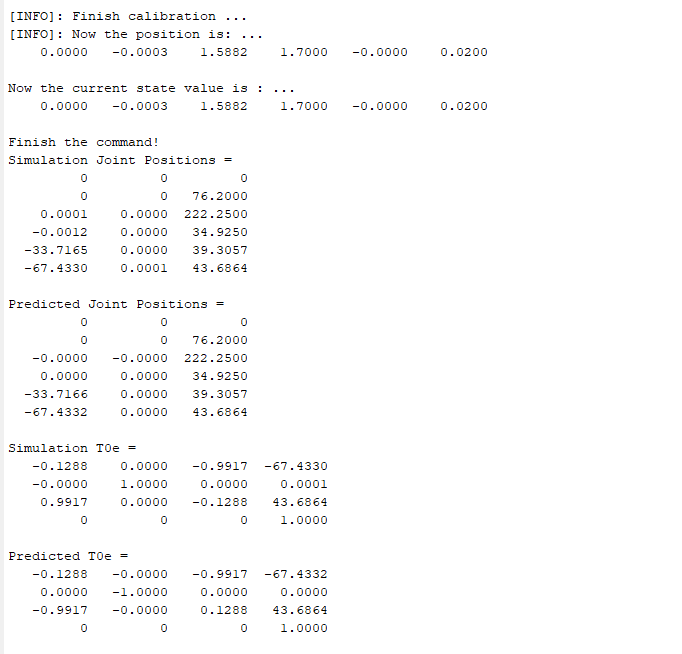
\includegraphics[scale=.5]{firstweird config}
\caption{First interesting configuration}
\end{figure}

\newpage
\par{
Another interesting point was entering the joint limit of every joint. We were hoping to see if gazebo misbehaved right at its dexterous workspace, but saw no such behavior. This was reassuring because it allows us to trust gazebo to handle inputs that approach or even go pass the joint limits.
}\\
\begin{figure} [h]
	\centering 
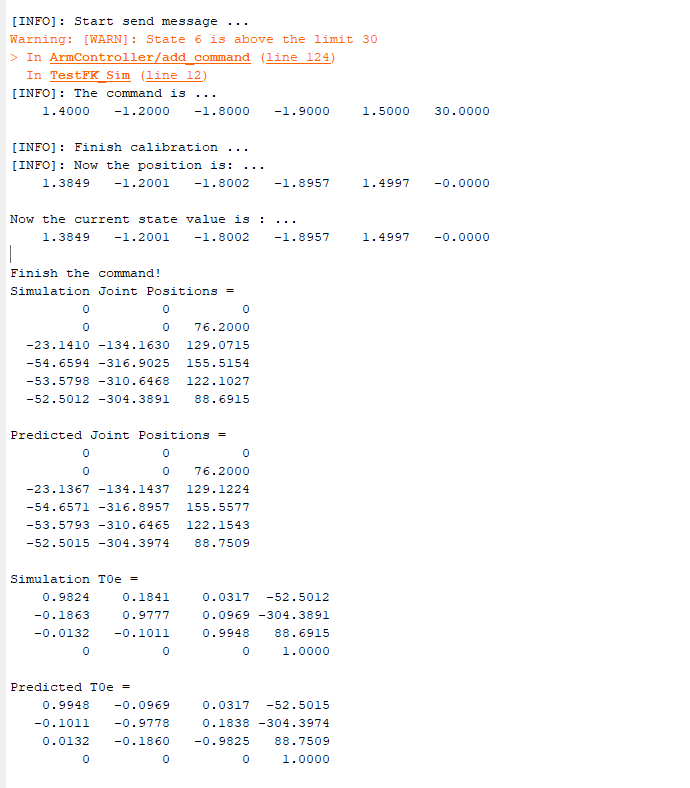
\includegraphics[scale=.5]{entering the joint limits of every joint}
\caption{Entering the joint limits of every joint}
\end{figure}
 \newpage
\par{
We also noticed that going over the joint limits causes our predicted values to deviate greatly. This is because Ros and gazebo prevent the joint from traveling further along each joint than is possible. However, our code does not account for going over the joint limits. As a result, entering -5 into $\theta_{2}$ as we did in our example causes our predicted end effector position to be significantly off.
}
\\
\begin{figure} [h!]
	\centering 
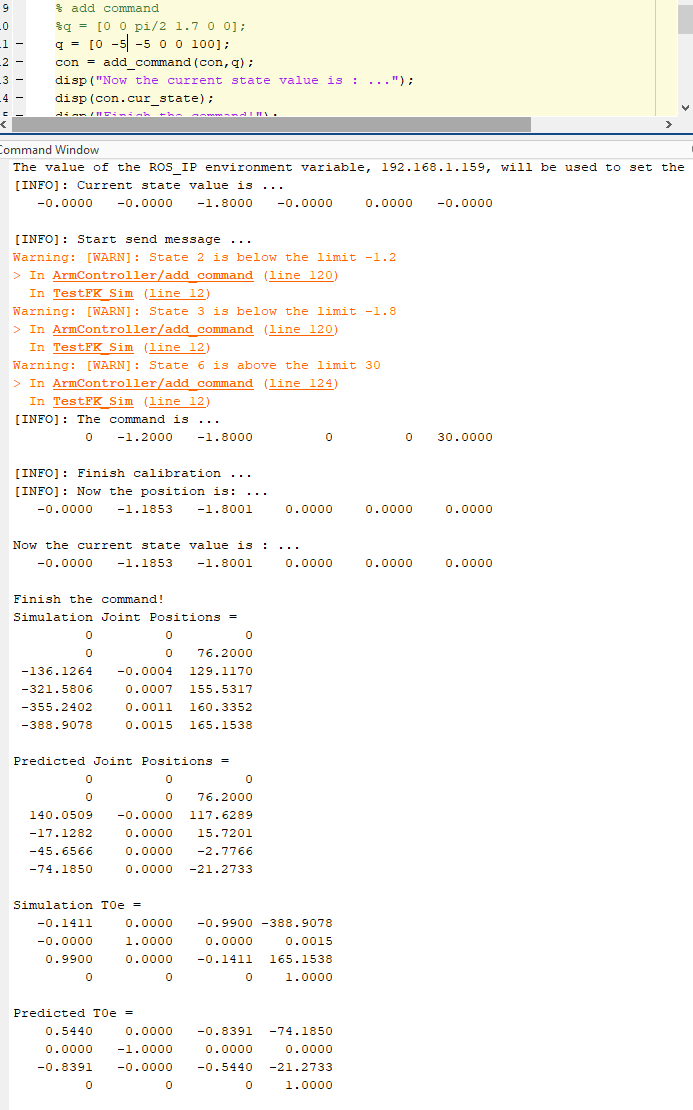
\includegraphics[scale=.4]{interesting q case}
\caption{Interesting q case}
\end{figure}


\newpage
\par{
This is a simple starting position, but we consider it an interesting point because if you look at the orientation that gazebo outputs you can clearly see that the z axis is incorrectly oriented. This is very important to know when evaluating the orientation of the end effector.
}\\
\begin{figure}  [h!]
	\centering 
\includegraphics[scale=.5]{inverted z axis }
\caption{Inverted z axis }
\end{figure}

\newpage
\par{
We chose to orient the arm straight up along the z axis. In gazebo we noticed that maintaining this orientation, seemed to be unstable and the arm continually swayed in the positive negative x direction. We found this very interesting,and became curious whether this is a result of simulated physics in ros.
}\\
\begin{figure} [h!]
	\centering 
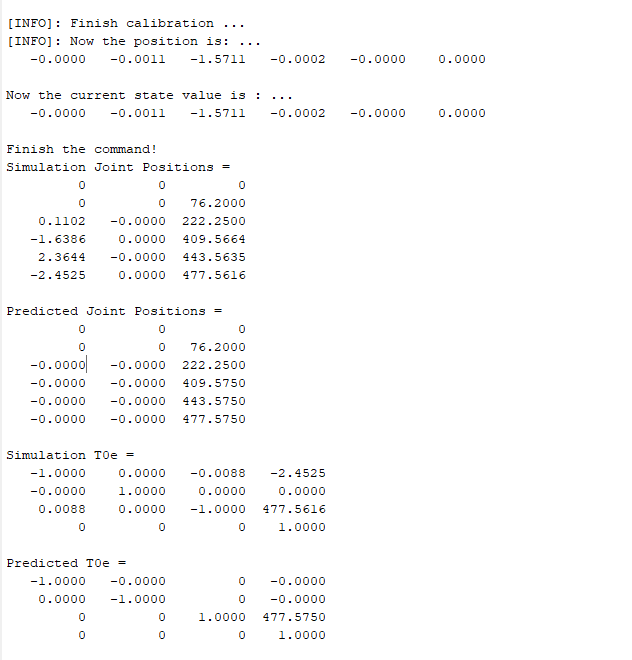
\includegraphics[scale=.5]{straight up}
\caption{Pointing straight up}
\end{figure}
\newpage
\item 
\par{Calculating the workspace was a matter of walking through the joint space. That is to say, that the permutation of all possible joint coordinates will give the entirety of the workspace. To implement this, we used 5 for loops, giving a time complexity of $O(n^{5})$. Instead of reducing the dimensionality of joint space to reduce the time complexity, we chose to use a larger step sizes as we walked through each dimension in joint space. This was feasible by using MATLAB's trisurf command that allowed us to plot a 3d surface with relatively few 3d points. To get the corresponding point in 3 dimensional space from a coordinate in joint space, we used the $T^{0}_{5(e)} $ that we calculated previously.  By inputting the joint parameters into $T^{0}_{5(e)}$ and pulling the final column of this homogeneous matrix, we were able to get a point in 3D that represented the location of the end effector given some joint parameters.}
\begin{figure} [h!]
	\centering 
	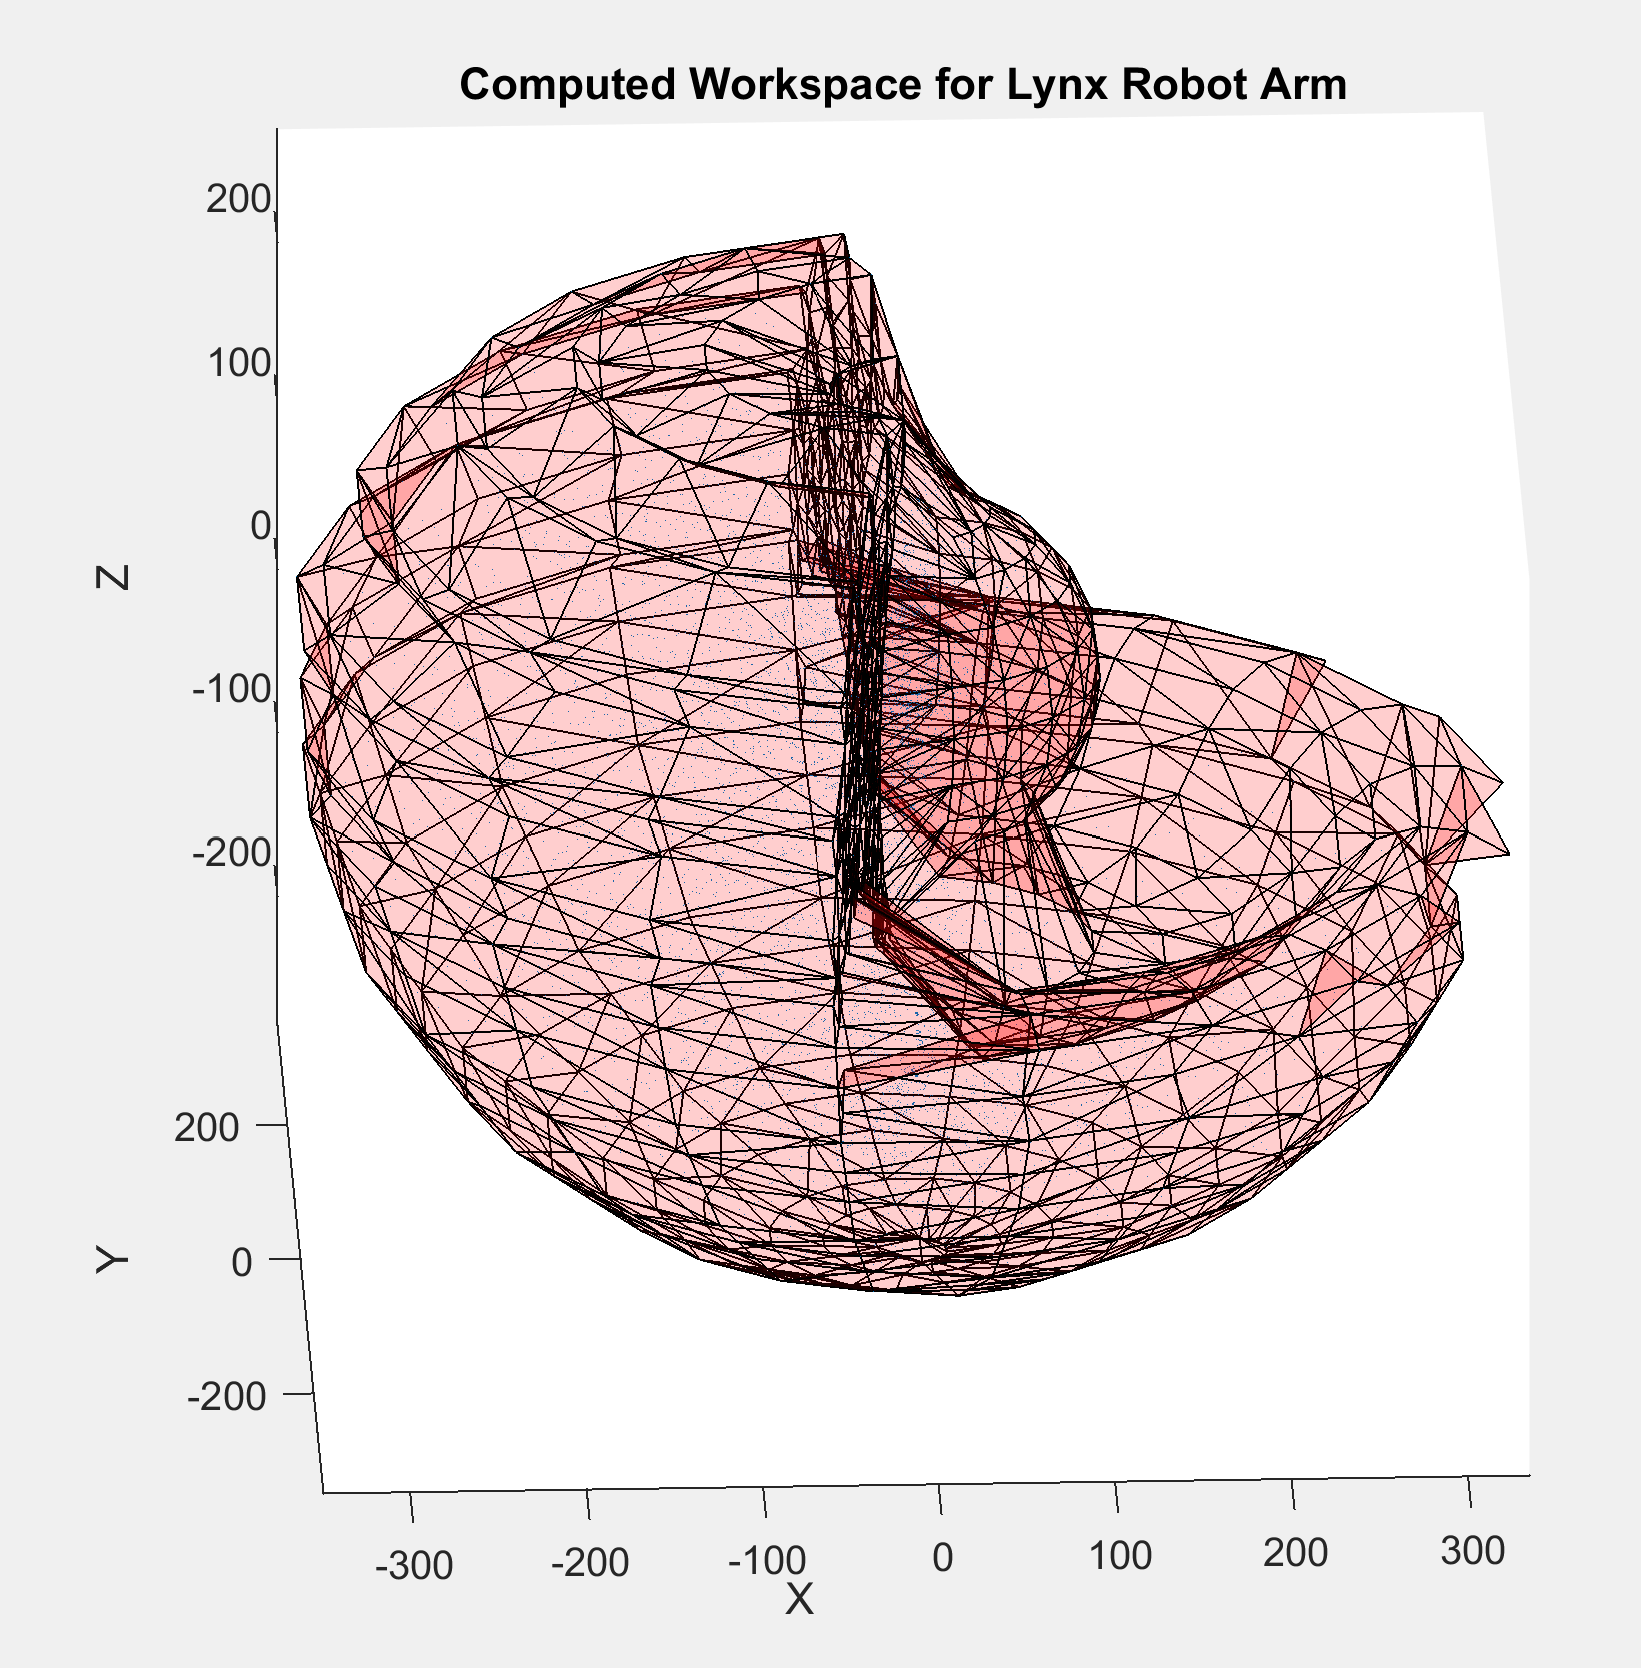
\includegraphics[scale=.5]{ComputedWorkspace.png}
	\caption{Computed Workspace of Lynx Robot}
	\end{figure}
	\newpage
\item As seen in the code below, the predicted joint positions are almost exactly aligned with the simulated joint positions, aside from a 0.002mm difference in the x position of Joint 3. This is negligible and can be explained due to possible compounded rounding errors in the ROS robot.\\ \\ However, when examining the $T^{0}_{e}$ matrices, the Simulation $T^{0}_{e}$ records different values of $x_{0}$ and $y_{0}$ in the end effector frame. We believe that this is due to a mistake in the provided ROS robot code used to calculate Simulation $T^{0}_{e}$. Justification for this conjecture is provided in Problem 1 of the Analysis section.\\

\lstinputlisting[style=Matlab-editor,caption={Outputs of TestFK\_Sim.m for 
	$q = \begin{bmatrix}
	0 & 0 & 0 & 0 & 0 & 0\\
	\end{bmatrix}$}]{24Prob5output.m}


\end{enumerate}

\newpage
\section{Analysis}
\begin{enumerate}
\item As expected, the results of our evaluation were correct. From the figure below, we use Right-Hand Rule convention to establish that the base frame's red axis is $x_{0}$, the green axis is $y_{0}$ and the blue axis is $z_{0}$. The same axes are applied to the end effector frame, respectively. \\\begin{figure} [h]
	\centering 
	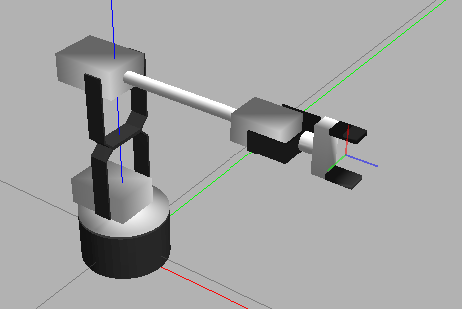
\includegraphics[scale=2]{ImageOfRobotZeroConfig.png}
	\caption{ROS Robot in Zero Configuration}
	\end{figure} \\
If we use these axes to construct a rotation matrix $R$ by observing each end effector's axis' projection on the base frame's axes, we can compute the following rotation matrix:
\\
\begin{equation}
R = \begin{bmatrix}
	0 & 0 & 1 \\
	0 & -1 & 0\\
	1 & 0 & 0
	\end{bmatrix}
\end{equation}
\\
For example, $R$ states that the projection of the end effector's y axis $y_{e}$ is in the opposite direction of the base frame's y axis $y_{0}$. This value validates the Predicted $T^{0}_{e}$ in Analysis Problem 2.4 and shows that the Simulated $T^{0}_{e}$ is incorrect.\\\\Fortunately, as seen in the same problem, the joint positions were not affected by this error.


\item 
\par{Yes, many points that would’ve collided with the frame of the robot are reachable in our predicted workspace. This occurred because neither Ros,Gazebo, or ourselves took collision into account. Withstanding those points, there were still points predicted as reachable, but were not actually reachable in the simulation. This is because our calculateFk did not take joint limits into account it only utilized the $T^{0}_{e}$. As a result, it was possible to input joint parameters that resulted in dramatically different results than the simulation, as long as those joint inputs were outside the designated joint limits defined by ros. A way to account for this would be to include joint limits in calculateFK. The inverse is not true; we did not find any points that were reachable in the simulation that were predicted as unreachable. The main sources or deviation from simulation and prediction was caused by not having sufficient checks of joint limits in calculateFk.}
\end{enumerate}
\section{Code Makeup}
\par{ The code essentially implements DH4 convention to find the coordinate frames of each joint and the end effector. We use a helper function called createA.m to create an $A^{i-1}_{i}$. This function takes in DH4 parameters and outputs the corresponding $A^{i-1}_{i}$ matrix . We then create another matrix that contains all the relevant DH4 parameters, and by walking though each row in the DH4 parameter matrix,inputing it into create A, and post multiplying we were able to get the intermediate frames and $T^{0}_{e}$. Using joint coordinates and $T^{0}_{e}$ gave us the location of the end effector and its orientation. Using this in combination with walking through each joint to create the workspace, and getting the joint location of each joint in the base frame was simple matter of post multiplying until you got to the frame containing the desired joint location. This final matrix gave both the orientation and location of the joint. The only exception was joint 4 because the coordinate frame did not exist on the joint; as a result, we had to multiply $T^{0}_{4}$ with the column vector $q=[0,0,L_{4},1]$ to translate the frame $T^{0}_{4}$  to the location of joint 4.
}

\section{Conclusion}
\par{This lab was an exercise in implementing forward kinematics, in the simulated ROS environment. Despite the the sophistication of Ros, there were noticeable deviations from reality. The main deviation was a result of collision. The Robot was able to collide with itself with absolutely no resistance. There were also cases where the robot did not directly collide with itself, but instead entered positions that most certainly would've torn wires present in the real robot. We also didn't control the speed of the robot and focused primarily on the kinematics. These considerations are important because when we eventually use a real robot we will need to consider these differences to prevent damaging physical systems.
}
\section{Appendix}
%\lstinputlisting[style=Matlab-editor,caption={calculateFK.m]{Code/calculateFK.m}
	
%\lstinputlisting[style=Matlab-editor,caption={computeWorkspace.m]{Code/computeWorkspace.m}
	
%\lstinputlisting[style=Matlab-editor,caption={createA.m]{Code/createA.m}
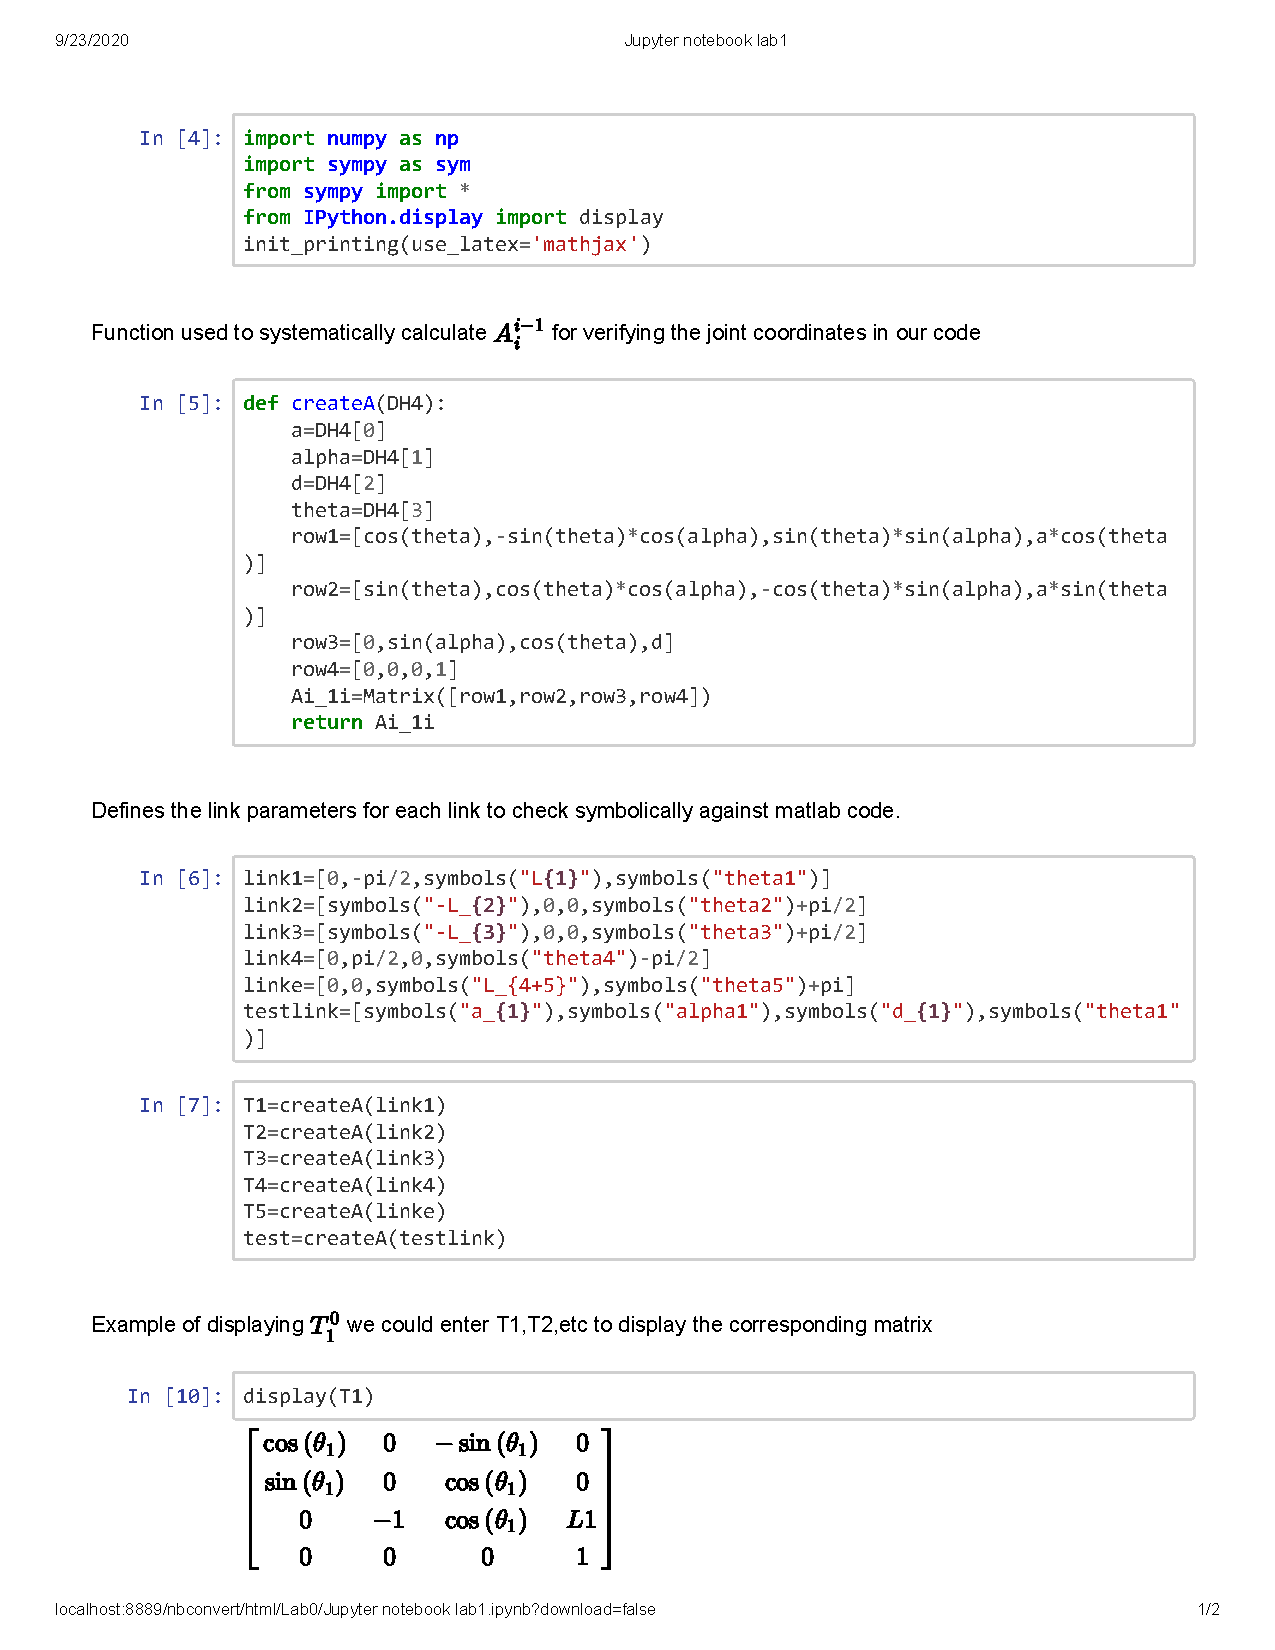
\includepdf[page=-]{Jupnotebook}
\end{document}
